\documentclass[coursework]{SCWorks}
% Тип обучения (одно из значений):
%    bachelor   - бакалавриат (по умолчанию)
%    spec       - специальность
%    master     - магистратура
% Форма обучения (одно из значений):
%    och        - очное (по умолчанию)
%    zaoch      - заочное
% Тип работы (одно из значений):
%    coursework - курсовая работа (по умолчанию)
%    referat    - реферат
%  * otchet     - универсальный отчет
%  * nir%ournal - журнал НИР
%  * digital    - итоговая работа для цифровой кафдры
%    diploma    - дипломная работа
%    pract      - отчет о научно-исследовательской работе
%    autoref    - автореферат выпускной работы
%    assignment - задание на выпускную квалификационную работу
%    review     - отзыв руководителя
%    critique   - рецензия на выпускную работу
% Включение шрифта
%    times      - включение шрифта Times New Roman (если установлен)
%                 по умолчанию выключен
\usepackage{preamble}
\begin{document}

% Кафедра (в родительном падеже)
\chair{математической кибернетики и компьютерных наук}

% Тема работы
\title{Реализация семантического поиска на корпусе новостных документов}

% Курс
\course{3}

% Группа
\group{351}

% Факультет (в родительном падеже) (по умолчанию "факультета КНиИТ")
% \department{факультета КНиИТ}

% Специальность/направление код - наименование
% \napravlenie{02.03.02 "--- Фундаментальная информатика и информационные технологии}
% \napravlenie{02.03.01 "--- Математическое обеспечение и администрирование информационных систем}
% \napravlenie{09.03.01 "--- Информатика и вычислительная техника}
\napravlenie{09.03.04 "--- Программная инженерия}
% \napravlenie{10.05.01 "--- Компьютерная безопасность}

% Для студентки. Для работы студента следующая команда не нужна.
% \studenttitle{Студентки}

% Фамилия, имя, отчество в родительном падеже
\author{Янченко Вадима Александровича}

% Заведующий кафедрой 
\chtitle{доцент, к.\,ф.-м.\,н.}
\chname{С.\,В.\,Миронов}

% Руководитель ДПП ПП для цифровой кафедры (перекрывает заведующего кафедры)
% \chpretitle{
%     заведующий кафедрой математических основ информатики и олимпиадного\\
%     программирования на базе МАОУ <<Ф"=Т лицей №1>>
% }
% \chtitle{г. Саратов, к.\,ф.-м.\,н., доцент}
% \chname{Кондратова\, Ю.\,Н.}

% Научный руководитель (для реферата преподаватель проверяющий работу)
\satitle{доцент, к.\,ф.-м.\,н.} %должность, степень, звание
\saname{С.\,В.\,Папшев}

% Руководитель практики от организации (руководитель для цифровой кафедры)
\patitle{доцент, к.\,ф.-м.\,н.}
\paname{С.\,В.\,Миронов}

% Руководитель НИР
\nirtitle{доцент, к.\,п.\,н.} % степень, звание
\nirname{В.\,А.\,Векслер}

% Семестр (только для практики, для остальных типов работ не используется)
\term{2}

% Наименование практики (только для практики, для остальных типов работ не
% используется)
\practtype{учебная}

% Продолжительность практики (количество недель) (только для практики, для
% остальных типов работ не используется)
\duration{2}

% Даты начала и окончания практики (только для практики, для остальных типов
% работ не используется)
\practStart{01.07.2022}
\practFinish{13.01.2023}

% Год выполнения отчета
\date{2025}

\maketitle

% Включение нумерации рисунков, формул и таблиц по разделам (по умолчанию -
% нумерация сквозная) (допускается оба вида нумерации)
\secNumbering

\tableofcontents

% Раздел "Обозначения и сокращения". Может отсутствовать в работе
% \abbreviations
% \begin{description}
%     \item ... "--- ...
%     \item ... "--- ...
% \end{description}

% Раздел "Определения". Может отсутствовать в работе
% \definitions

% Раздел "Определения, обозначения и сокращения". Может отсутствовать в работе.
% Если присутствует, то заменяет собой разделы "Обозначения и сокращения" и
% "Определения"
% \defabbr

\intro
В современном мире объём текстовой информации стремительно растёт: ежедневно публикуются миллионы новостных статей, научных публикаций, блогов и других текстов. Это приводит к тому, что извлечение релевантной информации становится всё более сложной и ресурсоёмкой задачей. Особенно остро данная проблема стоит в сфере новостной аналитики, где важно не просто находить тексты по ключевым словам, но и понимать их смысл, контекст и скрытые связи между понятиями. В условиях информационного перенасыщения возрастает потребность в инструментах, которые способны анализировать тексты не только на уровне лексики, но и на уровне семантики.

Классические подходы к поиску информации, такие как полнотекстовый поиск, не всегда обеспечивают необходимый уровень точности и полноты, особенно в случае, когда пользовательский запрос выражен не теми словами, которые используются в целевых документах. Это может происходить из-за синонимии, омонимии, различий в стилистике и формулировках. В результате возникает необходимость в применении более интеллектуальных методов обработки естественного языка, которые позволяют учитывать смысловую близость слов и фраз.

Одним из наиболее перспективных направлений в области анализа текстов является использование эмбеддингов "--- векторных представлений слов, фраз и даже целых документов. Такие представления позволяют преобразовать текстовую информацию в числовой вид, сохраняющий семантические связи между элементами текста. Эмбеддинги, полученные с помощью моделей Word2Vec и GloVe, широко используются в задачах классификации, кластеризации, тематического моделирования и, в том числе, в семантическом поиске.

Семантический поиск, в отличие от традиционного, основывается не на простом совпадении слов, а на вычислении смысловой близости между запросом и содержанием документов. Это позволяет находить более релевантные результаты, учитывать контекст и преодолевать ограничения, связанные с различиями в формулировках. Особенно актуальным это становится в работе с новостными данными, где важна оперативность, полнота и точность информационного поиска.

Эмбеддинги, полученные с помощью моделей, которые обучены на огромном корпусе документов, например, Национальном корпусе русского языка (НКРЯ), обладают высокой универсальностью и охватывают широкий спектр лексических и синтаксических конструкций. Однако такие модели формируют обобщённые представления слов и выражений, которые отражают усреднённые языковые закономерности, присущие общему языку. В результате они не способны в полной мере учитывать специфику отдельных предметных областей.
Поэтому необходимо использовать эмбеддинги, обученные или дообученные на специализированных корпусах, отражающих специфику выбранной тематики "--- в данном случае новостных текстов.

Таким образом, возникает проблема в создании модели, которая бы отражала наиболее полно предметную область, и, как следствие, лучше всего отвечала на запросы пользователей. 

Цель курсовой работы "--- разработать систему семантического поиска по корпусу новостных документов на основе эмбеддингов.

Для достижения поставленной цели необходимо решить следующие задачи:
\begin{enumerate}
    \item изучить теоретические основы построения векторных представлений слов и документов, а также ознакомиться с архитектурами моделей Word2Vec и GloVe, исследовать понятие тезауруса и методы его формирования на основе эмбеддингов;

    \item построить модели Word2Vec и GloVe на корпусе новостных документов и проанализировать их;

    \item разработать алгоритм семантического поиска;

    \item провести сравнительный анализ моделей Word2Vec и GloVe в контексте задачи семантического поиска.
\end{enumerate}

\section{Алгоритмы построения эмбеддингов}
В контексте обработки естественного языка слова рассматриваются как элементы, обладающие лексико-семантическими характеристиками. Базовой единицей анализа выступает лемма "--- начальная форма слова. От неё образуются различные словоформы, отражающие морфологические изменения (например, \textit{дом} "--- \textit{дома}, \textit{дому} и т.д.).

Одна лемма может иметь несколько значений "--- это явление, известное как полисемия. Это затрудняет однозначную интерпретацию и требует учёта контекста. Кроме того, в языке существуют слова близкие по значению "--- синонимы. Классическим формальным критерием синонимии считается взаимозаменяемость слов в высказывании без изменения его условий истинности. Однако на практике полная синонимичность встречается редко: лексемы могут различаться стилистически (например, \textit{жена} "--- \textit{супруга}) или семантически по оттенкам (\textit{мокрый} "--- \textit{влажный}).

Помимо синонимии важную роль играет сходство слов "--- более общее понятие, не предполагающее полной тождественности значений. Например, кошка и собака "--- не синонимы, но они семантически близки по ряду признаков (домашние животные, млекопитающие и т.д.). Анализ сходства между словами позволяет работать на уровне поверхностной лексики, не опираясь на формальные модели значений, что существенно упрощает вычислительную обработку.

Мера лексического сходства используется в широком спектре задач "--- от оценки семантической близости слов и фраз до построения более сложных моделей смыслового соответствия между предложениями и текстами. Именно на этих принципах основывается построение векторных представлений слов (эмбеддингов), где слова отображаются в пространстве таким образом, что семантически близкие слова располагаются ближе друг к другу.

Ключевая идея состоит в представлении слова как вектора в многомерном пространстве. Самый простой способ перехода от слова к вектору состоит в следующем: пусть $V$ "--- множество всех слов. Слово $w_i \in V$ представим как вектор размера $n = |V|$, в котором все координаты равны $0$ кроме $i$"=ой координаты, которая равна $1$\cite{jm3}.

\subsection{Алгоритм модели Word2Vec}
Рассмотрим другой способ представления слова как вектора "--- эмбеддинг. Эмбеддинги имеют количество размерностей $d$ от 50 до 1000, что существенно меньше количества слов $|V|$ во всех документах. Кроме того, эти векторы плотные: вместо того, чтобы большинство координат были равны 0, значения будут вещественными числами, которые могут быть и отрицательными\cite{wang2019evaluating}.

Эмбеддинги Word2Vec являются статическими, это означает, что каждому слову соответствует ровно один эмбеддинг. Такие модели как BERT, основанные на архитектуре трансформеров, позволяют создавать контекстуальные эмбеддинги, которые сопоставляют разный вектор к слову в зависимости от контекста\cite{vaswani2017attention}.

Модель Word2Vec реализуется в двух основных архитектурах: CBOW и Skip"=Gram.

\subsubsection{Архитектура модели Skip-Gram}

Модель Skip-Gram является одной из двух основных архитектур Word2Vec и направлена на предсказание контекстных слов по центральному слову. То есть, имея слово $w_t$, модель обучается предсказывать слова, находящиеся в некотором окне вокруг него: $w_{t-c}, \dots, w_{t-1}, w_{t+1}, \dots, w_{t+c}$, где $c$ "--- размер окна\cite{church2017word2vec}.


Модель Skip-Gram представляет собой простую нейросеть с одним скрытым слоем. Она состоит из следующих компонентов:

\begin{enumerate}
  \item Входной слой.
  Каждое слово из словаря $V$ кодируется как one-hot вектор $\mathbf{x} \in \mathbb{R}^{|V|}$, в котором все элементы равны нулю, кроме одного, соответствующего индексу слова $w$.

  \item Скрытый слой.
  Представлен матрицей весов $W \in \mathbb{R}^{|V| \times d}$, где $d$ "--- размерность эмбеддингового пространства. Преобразование входа:
  \[
  \mathbf{h} = \mathbf{x}^\top W
  \]
  Вектор $\mathbf{h} \in \mathbb{R}^d$ и является искомым эмбеддингом слова $w$.

  \item Выходной слой. 
  Представлен второй матрицей весов $W' \in \mathbb{R}^{d \times |V|}$. Результат выходного слоя:
  \[
  \mathbf{u} = W'^\top \mathbf{h}
  \]
  где $\mathbf{u} \in \mathbb{R}^{|V|}$ "--- логиты для каждого слова в словаре.

  \item Softmax.
  На выходе применяется softmax-функция, преобразующая логиты в вероятности:
  \[
  P(w_O \mid w_I) = \frac{\exp(\mathbf{v}'_{w_O} \cdot \mathbf{v}_{w_I})}{\sum_{w \in V} \exp(\mathbf{v}'_w \cdot \mathbf{v}_{w_I})}
  \]
  Здесь:
  \begin{itemize}
    \item $w_I$ "--- входное (центральное) слово;
    \item $w_O$ "--- слово из контекста;
    \item $\mathbf{v}_{w_I}$ "--- вектор из матрицы $W$ (входной эмбеддинг);
    \item $\mathbf{v}'_{w_O}$ "--- вектор из матрицы $W'$ (выходной эмбеддинг).
  \end{itemize}
\end{enumerate}

Рассмотрим функцию потерь.
Для одного примера $(w_I, w_O)$ используется кросс-энтропия:
\[
\mathcal{L} = -\log P(w_O \mid w_I)
\]
Общая функция потерь по корпусу:
\[
\mathcal{L}_{\text{total}} = -\sum_{t=1}^{T} \sum_{\substack{-c \leq j \leq c \\ j \ne 0}} \log P(w_{t+j} \mid w_t)
\]
где $T$ "--- длина корпуса.

Эмбеддингом является как матрица ($W$), так и матрица($W'$) "--- часто используется только $W$. 

Стоит отметить, что несмотря на отсутствие явного задания семантики при обучении, модели типа Word2Vec способны выявлять семантические закономерности на основе статистических свойств текстового корпуса. Это объясняется тем, что модели обучаются на контекстных соотношениях между словами, отражающих их типичную совместную встречаемость.

Характерный пример — аналогичные отношения между словами: векторное представление слова «королева» может быть получено как результат векторной операции: король $-$ мужчина $+$ женщина $=$ королева, где каждое слово представляется как эмбеддинг\cite{jatnika2019word2vec}.

Другой пример: отношение «мужчина» : «женщина» аналогично отношению «дядя» : «тётя». Такие примеры иллюстрируют способность модели захватывать не только лексическую, но и семантическую структуру языка на уровне распределения контекстов\cite{vylomova2015take}.

Полноценный расчёт softmax-функции в модели Skip-Gram требует вычисления скалярного произведения с каждым словом в словаре, что приводит к высокой вычислительной сложности: $\mathcal{O}(|V|)$ на каждый пример.
Для решения этой проблемы в модели Word2Vec используется приближённый метод оптимизации "--- negative sampling.
  
\subsection{Алгоритм модели GloVe}

Модель GloVe (Global Vectors) предназначена для построения векторных представлений слов на основе глобальной статистики совместных появлений слов в тексте. В отличие от моделей Word2Vec, которые обучаются на локальных контекстных окнах, GloVe использует информацию о числе совместных появлений слов во всём корпусе, агрегируя её в специальную матрицу.

На первом этапе строится матрица совместных появлений $X \in \mathbb{R}^{|V| \times |V|}$, где $X_{ij}$ "--- количество раз, когда слово $j$ встречается в контексте слова $i$. Контекст обычно ограничивается окном фиксированного размера (например, 5 слов влево и вправо), при этом можно учитывать взвешивание по расстоянию до центрального слова\cite{pennington2014glove}.

GloVe обучает два векторных представления: $w_i \in \mathbb{R}^d$ "--- для центрального слова $i$ и $\tilde{w}_j \in \mathbb{R}^d$ "--- для контекстного слова $j$, а также два скалярных смещения $b_i$ и $\tilde{b}_j$. Обучение направлено на аппроксимацию следующего равенства:

\[
w_i^\top \tilde{w}_j + b_i + \tilde{b}_j \approx \log X_{ij}
\]

Целевая функция, которую минимизирует модель, записывается в следующем виде:

\[
J = \sum_{i=1}^{|V|} \sum_{j=1}^{|V|} f(X_{ij}) \left(w_i^\top \tilde{w}_j + b_i + \tilde{b}_j - \log X_{ij} \right)^2
\]

где $f(X_{ij})$ "--- весовая функция, ограничивающая влияние часто встречающихся пар слов, например:

\[
f(x) = 
\begin{cases}
\left(\frac{x}{x_{\text{max}}}\right)^\alpha & \text{если } x < x_{\text{max}} \\
1 & \text{иначе}
\end{cases}
\]

На практике используются значения $\alpha = 0{,}75$ и $x_{\text{max}} = 100$\cite{pennington2014glove}.

% Обучение проводится методом стохастического градиентного спуска или его модификаций (например, AdaGrad). На каждом шаге параметры $w_i$, $\tilde{w}_j$, $b_i$, $\tilde{b}_j$ обновляются таким образом, чтобы минимизировать ошибку между скалярным произведением векторов и логарифмом числа совместных появлений.

После завершения обучения итоговое представление слова $i$ получается как сумма обученных векторов:

\[
v_i = w_i + \tilde{w}_i
\]

Таким образом, каждая лексема кодируется плотным вектором фиксированной размерности, отражающим её глобальные статистические связи с другими словами корпуса.


% Word2Vec фокусируется на локальном контексте, обучаясь на парах центр-контекст, и опирается на информацию из небольших окон. В отличие от неё, GloVe использует глобальную статистику словоупотребления по всему корпусу, строя векторные представления на основе матрицы ко-частотности (co-occurrence matrix) "--- то есть того, насколько часто слова встречаются рядом друг с другом.

% Это позволяет GloVe более явно учитывать семантические связи между словами, которые могут не быть очевидными в локальных контекстах.

% Мб добавить + PMI
% \subsection{Контекстуальные модели. BERT}


\section{Понятие информационно-поискового тезауруса}
В информационном поиске широко используется механизм расширения запроса, основанный на добавлении семантически связанных терминов. Это позволяет находить релевантные документы, даже если в них отсутствуют исходные ключевые слова.

Для определения связанных по смыслу слов применяется тезаурус — лексический ресурс, фиксирующий семантические отношения между словами (синонимия, антонимия, гипонимия и др.). В отличие от обычных словарей, тезаурусы структурируют связи между терминами\cite{thesaurus}.

Тезаурусы бывают экспертными и автоматически построенными с помощью статистических и нейросетевых методов. Последние особенно важны для областей с быстро меняющейся лексикой таких, как новостные тексты.

Один из наиболее известных тезаурусов "--- WordNet, содержащий около $155000$ лексем, организованных в синсеты (совокупности синонимов). В WordNet синонимы считаются взаимозаменяемыми, если замена не меняет значения высказывания хотя бы в некоторых контекстах\cite{miller1995wordnet}.


\section{Семантический поиск}
Семантический поиск "--- это современный этап эволюции систем информационного поиска, основной задачей которого является не просто нахождение документов, содержащих заданные пользователем слова, а выявление наиболее смыслосообразных и релевантных результатов. Суть этого подхода заключается в том, чтобы приблизить машинное восприятие текста к человеческому пониманию, опираясь не только на внешнюю форму запроса, но и на его содержание, контекст и предполагаемое значение.

На протяжении десятилетий традиционные поисковые алгоритмы основывались на прямом сопоставлении слов из пользовательского запроса с документами. Такой подход, хоть и прост в реализации, имеет ряд существенных ограничений, особенно в тех случаях, когда пользователь использует неточные формулировки, обобщённые термины или специфические выражения. В реальности человек крайне редко формулирует свой запрос с использованием тех же терминов, которые использованы в документе. Это создает разрыв между запросом и ответом, который семантический поиск стремится преодолеть.

Семантический поиск позволяет выходить за пределы лексического уровня языка, поднимаясь на уровень смысла и понятий. Это означает, что система стремится не к буквальному, а к содержательному совпадению. Происходит своего рода «перевод» текста на универсальный язык смыслов, в котором сравнение осуществляется не между словами, а между их внутренними представлениями. Таким образом, даже если запрос и документ имеют разную формулировку, они могут быть распознаны как близкие по значению\cite{search}.

\subsection{Алгоритм работы семантического поиска}
Семантический поиск основывается на идее сопоставления смыслового содержания запроса и документов, а не их поверхностного совпадения по ключевым словам. В основе его работы лежит представление текста в виде векторных эмбеддингов, отражающих значения слов, фраз или целых предложений в числовой форме.

Классическая схема семантического поиска включает несколько ключевых этапов:
\begin{enumerate}
    \item Предварительная обработка текста.
    
На этом этапе происходит очистка текста, токенизация, приведение слов к базовой форме (лемматизация), а также удаление второстепенных элементов вроде стоп-слов. Это стандартный этап, подготавливающий данные к последующему преобразованию в вектора.

    \item Преобразование в эмбеддинги.
    
И запрос, и документы кодируются векторными представлениями с помощью заранее обученной модели. Эти векторы отражают смысл текста и располагаются в общем семантическом пространстве, где близкие по значению тексты имеют схожие координаты.

    \item Вычисление сходства.
    
После получения эмбеддингов производится сравнение запроса с документами. Как правило, используется косинусное сходство "--- метрика, измеряющая угол между векторами. Чем ближе векторы, тем выше семантическая релевантность.

    \item Ранжирование результатов.
    
Документы сортируются по степени семантической близости к запросу. Дополнительно могут использоваться фильтры, бизнес-логика, временные ограничения и прочие факторы для уточнения выдачи.
\end{enumerate}

\subsection{Формирование и хранение эмбеддингов документов}

Для реализации семантического поиска необходимо, чтобы как пользовательские запросы, так и документы, по которым осуществляется поиск, были представлены в виде векторных эмбеддингов. Эмбеддинг документа "--- это числовое представление его смыслового содержания в виде вектора фиксированной размерности. Такой вектор позволяет сравнивать документ с другими объектами в пространстве признаков и находить наиболее близкие по смыслу тексты\cite{ye2016word}.

\subsubsection{Получение эмбеддингов документов}
Эмбеддинги документов могут быть получены разными способами, в зависимости от используемой языковой модели:
\begin{itemize}
    \item 
    Среднее по эмбеддингам слов: один из простейших подходов, когда для каждого слова в документе берётся эмбеддинг (например, с использованием Word2Vec или GloVe), а затем рассчитывается среднее значение по всем словам. Такой метод работает быстро, но теряет информацию о порядке слов и контексте.
    
    \item Модели предложений и документов: современные модели, такие как BERT и его производные, позволяют получать контекстно-зависимые представления целых предложений или документов. Обычно для этого используется [CLS]-токен (в случае BERT) или пуллинг эмбеддингов по всем токенам. Такие представления дают более точную оценку смысла текста.
    
    \item Фиксация эмбеддингов: после того как эмбеддинг для каждого документа получен, его можно сохранить отдельно от исходного текста, чтобы в дальнейшем не производить повторных вычислений.
\end{itemize}

\subsubsection{Хранение эмбеддингов документов}
Поскольку при семантическом поиске основная задача "--- быстро найти векторы, близкие к вектору запроса, необходимо эффективное хранение эмбеддингов и поддержка операций поиска по векторному пространству.

Существует несколько практических подходов к хранению эмбеддингов:
\begin{enumerate}
    \item
Наиболее простой способ "--- сохранить эмбеддинги в виде обычных массивов чисел (например, в формате \verb|.npy|, \verb|.json|, \verb|.csv|) и сопоставить их с идентификаторами документов. Это может подойти для небольших коллекций, но неэффективно для быстрого поиска: при каждом запросе придётся сравнивать вектор запроса с каждым вектором в базе.

    \item Чтобы обеспечить масштабируемость и быстродействие, эмбеддинги сохраняются в специальных индексных структурах, предназначенных для приближённого поиска ближайших векторов (ANN "--- Approximate Nearest Neighbors). Такие индексы позволяют значительно сократить количество сравниваемых векторов за счёт предварительной организации данных.

Наиболее популярные технологии:
\begin{itemize}
    \item 
    FAISS (Facebook AI Similarity Search)
    Библиотека от Facebook, которая позволяет создавать и хранить векторные индексы, включая кластеризацию, квантование и сокращение размерности. Поддерживает хранение миллионов векторов и эффективный поиск по ним.

    \item HNSW (Hierarchical Navigable Small World)
    Графовая структура, которая обеспечивает быстрый и точный поиск ближайших соседей. Поддерживается в библиотеках, таких как nmslib, annoy, и плагинах для Elasticsearch и других систем.
\end{itemize}

    \item Для продвинутых приложений используются специализированные СУБД, разработанные специально для хранения и обработки эмбеддингов:
    \begin{itemize}
        \item 
        Pinecone "--- облачная векторная БД, поддерживающая миллионы объектов, масштабирование и фильтрацию.

        \item Weaviate "--- векторная СУБД с возможностью выполнять семантический поиск и хранить связанные метаданные.

        \item Milvus "--- высокопроизводительная open-source система для работы с векторами.
        \end{itemize}
\end{enumerate}

% \subsection{Расширение запроса}

% Часто пользователь формулирует запрос слишком кратко, не используя все возможные синонимы, родственные понятия или специфические термины, которые присутствуют в искомой информации. Расширение запроса (Query Expansion) позволяет решить эту проблему. Оно позволяет:
% \begin{itemize}
%     \item Увеличить охват: за счёт добавления близких по смыслу слов система сможет найти документы, в которых используются другие формулировки.
    
%     \item Повысить релевантность: расширение позволяет точнее отразить смысл запроса, учитывая контекст и вариативность языка.
    
%     \item Снизить проблему разнородности терминологии: разные авторы могут описывать одни и те же явления разными словами.
% \end{itemize}

% Основные подходы к расширению запроса
% Ручное расширение
% Пользователь сам дополняет запрос дополнительными словами или уточнениями. Это наименее автоматизированный способ и зависит от компетентности и желания пользователя.

% Один из способов автоматического расширения основан  на применении тезаурусов.
% Система использует заранее подготовленные ресурсы "--- синонимические ряды, онтологии, словари, чтобы добавить к запросу близкие по смыслу слова или термины. Например, к слову <<автомобиль>> могут быть добавлены <<машина>>, <<транспорт>> и т.п.

\section{Разработка системы семантического поиска}
Весь программный код написан на языке программирования python версии $3.12.6$. В программном коде используются следующие библиотеки:
\begin{itemize}
  \item pandas для удобного управления данными;
  \item dask как быстрая альтернатива pandas, так как распараллеливает вычисления;
  \item natasha для предварительной обработки текста;
  \item gensim для работы с моделями;
  \item networkx для работы с графами;
  \item faiss для семантического поиска.
\end{itemize}

Ознакомиться со всем проектом можно в репозитории\footnote{https://github.com/Mindero/Thesaurus-construction} в github.
\subsection{Предварительная обработка данных}
Рассмотрим данные, которые представляют из себя новости, взятые из официального сайта СГУ. Каждый документ характеризуется следующими параметрами:
\begin{itemize}
  \item уникальный идентификатор новости;
  \item заголовок новости;
  \item необработанный текст новости;
  \item обработанный текст новости.
\end{itemize}

В таблице \ref{tab:data-example} приведён пример представления одной из новостей в используемом формате.

\begin{table}[!ht]
    \centering
    \footnotesize
    \begin{tabular}{|l|l|l|l|}
        \hline
        \multicolumn{1}{|c|}{\textbf{News\_Id}} & \multicolumn{1}{c|}{\textbf{News\_Title}}                                                                                & \multicolumn{1}{c|}{\textbf{News\_Text}}                                                                                   & \multicolumn{1}{c|}{\textbf{News\_Tokens}}                                                                                                                                                                                                                                 \\ \hline
        1                                       & \begin{tabular}[c]{@{}l@{}}Студенты и сотрудники \\ СГУ присоединились к \\ шествию «Бессмертного \\ полка»\end{tabular} & \begin{tabular}[c]{@{}l@{}}9 мая состоялась общенародная \\ акция «Бессмертный полк», \\ в которой приняли...\end{tabular} & \begin{tabular}[c]{@{}l@{}}{[}"май состояться общенародный \\    акция бессмертный полк \\    который принять участие \\    студент сотрудник",\\  "два год ограничение \\    пандемия долгожданный шествие \\    проходить традиционный формат", \\   ...{]}\end{tabular} \\ \hline
    \end{tabular}
    \caption{Пример представления одной из новостей в используемом формате}
    \label{tab:data-example}
\end{table}

Для получения обработанного текста выполняются следующие этапы:
\begin{enumerate}
    \item Удаление стоп"=слов.
    \item Лемматизация слов.
    \item Удаление имен людей, городов, стран, наименования различных компаний.
\end{enumerate}

Стоп-слова "--- это слова, которые встречаются в языке чрезвычайно часто, но, как правило, не несут самостоятельной смысловой нагрузки в контексте информационного поиска или анализа текста. К таким словам относятся, например, союзы, предлоги, частицы, местоимения: «и», «в», «на», «что», «как», «это», и т.п. Их исключение позволяет снизить «шум» в текстах, повысить эффективность алгоритмов и сосредоточиться на лексемах, действительно значимых для понимания содержания документа.
  
Лемматизация, в свою очередь, представляет собой процесс приведения слова к его начальной, словарной форме "--- лемме. Это позволяет уменьшить количество уникальных словоформ в тексте, объединив различные грамматические формы одного и того же слова (например, «пошёл», «идёт», «шли» "--- к лемме «идти»). Благодаря лемматизации повышается точность анализа, поскольку слова с одинаковым значением, но разными формами, будут обрабатываться как единое понятие.

Программный код, выполняющий обработку текста, можно рассмотреть в приложении \ref{apx:tokenization}.

Ознакомиться со статистикой полученных данных можно в табл. \ref{table:preprocess}.
\begin{table}[!h]
    \centering
    % \footnotesize
    \begin{tabular}{|l|l|}
    \hline
    \multicolumn{1}{|c|}{\textbf{Статистика}}  & \multicolumn{1}{c|}{\textbf{Значение}} \\ \hline
    Количество новостей                        & 31077                                  \\ \hline
    Общее количество предложений               & 423175                                 \\ \hline
    Среднее количество предложений на новость  & 13.62                                  \\ \hline
    Общее количество токенов                   & 4293732                                \\ \hline
    Среднее количество токенов на новость      & 138.16                                 \\ \hline
    Максимальное количество токенов на новость & 166                                    \\ \hline
    Минимальное количество токенов на новость  & 1                                      \\ \hline
    Количество уникальных токенов              & 45204                                  \\ \hline
    \end{tabular} 
    \caption{Статистика по полученным данным}
    \label{table:preprocess}
\end{table}

\subsection{Построение моделей на основе корпуса новостных документов}
\subsubsection{Построение модели Word2Vec}
\label{section:word2vec-construction}
Обучим модель Word2Vec на обработанных текстах новостей. В качестве входа новостей будут подаваться предложения, размер получаемых эмбеддингов равен $300$, а размер окна $5$. Кроме этого, будут исключены слова, которые встречаются менее $5$ раз, потому что эмбеддинги таких слов не будут отражать смысл этого слова. Программный код, выполняющий это, рассположен ниже.
\begin{minted}{python3}
import dask.dataframe as dd
import dask.bag as db
from gensim.models import Word2Vec
docs = dd.read_parquet("../output.pq/")
texts = docs['News_Tokens'].compute()
bag = db.from_sequence(texts)
sentences = bag.flatten().map(lambda x: x.split()).compute()
model = Word2Vec(sentences=sentences, vector_size=300, window=5,min_count=5, sg=0)
model.save('word2vec_sent_5_sgu.model')
\end{minted}

Результатом обучения будет бинарный файл, в котором к каждому слову представлен эмбеддинг.

Получив модель, построим тезаурус. Ознакомиться с кодом, выполняющий это можно в приложении \ref{apx:thesaurus}. В качестве результата получим таблицу, в которой каждая строка имеет вид: слово и его ближайшие синонимы. Отношение близости между синонимами в построенном тезаурусе не менее $0.7$, что является хорошей отсечкой для удаления некорректных результатов модели и шума.

Первые 10 строчек полученного файла отражены в табл. \ref{table:word2vec-example}. Второй элемент в паре равен косинусному расстоянию между словами.
\begin{table}[!h]
    \centering
    \small
    \begin{tabular}{|l|l|}
        \hline
        \multicolumn{1}{|c|}{\textbf{Word}} & \multicolumn{1}{c|}{\textbf{Most\_Similar\_Word}}                                                                                                                                                                                                                                                                                                          \\ \hline
        май                                 & \begin{tabular}[c]{@{}l@{}}{[}('апрель', 0.8788188099861145), ('февраль', 0.8743687272071838), \\  ('ноябрь', 0.8666709661483765), ('октябрь', 0.864989161491394), \\  ('декабрь', 0.855202317237854), ('январь', 0.8505667448043823), \\  ('июнь', 0.842693567276001), ('март', 0.8332036137580872), \\  ('сентябрь', 0.8205611705780029){]}\end{tabular} \\ \hline
        состояться                          & {[}('пройти', 0.8456324934959412){]}                                                                                                                                                                                                                                                                                                                       \\ \hline
        акция                               & {[}{]}                                                                                                                                                                                                                                                                                                                                                     \\ \hline
        бессмертный                         & {[}('полк', 0.9408268928527832){]}                                                                                                                                                                                                                                                                                                                         \\ \hline
        полк                                & {[}('бессмертный', 0.9408268928527832){]}                                                                                                                                                                                                                                                                                                                  \\ \hline
        который                             & {[}{]}                                                                                                                                                                                                                                                                                                                                                     \\ \hline
        принять                             & {[}('принимать', 0.8362864255905151){]}                                                                                                                                                                                                                                                                                                                    \\ \hline
        участие                             & {[}{]}                                                                                                                                                                                                                                                                                                                                                     \\ \hline
        студент                             & {[}{]}                                                                                                                                                                                                                                                                                                                                                     \\ \hline
    \end{tabular}
    \caption{Первые 10 строчек тезауруса, построенного моделью Word2Vec}
    \label{table:word2vec-example}
\end{table}
\subsubsection{Построение модели GloVe}
Для создания модели GloVe склонируем их официальный репозиторий\footnote{https://github.com/stanfordnlp/GloVe}. Далее выполним следующие команды, которые создают эмбеддинги для каждого слова:
\begin{minted}{bash}
build/vocab_count -min-count 5 -verbose 2 < corpus.txt > vocab.txt
build/cooccur -memory 4.0 -vocab-file vocab.txt -verbose 2 -window-size 7 < corpus.txt >cooccurrence.bin
build/shuffle -memory 4.0 -verbose 2 < cooccurrence.bin > cooccurrence.shuf.bin
build/glove -save-file vectors -threads 12 -input-file cooccurrence.shuf.bin -x-max 10 -iter 15 -vector-size 300 -binary 2 -vocab-file vocab.txt -verbose 2
\end{minted}

Модель строится по тем же параметрам, что и Word2Vec, а именно:
\begin{itemize}
    \item размер эмбеддинга равен $300$;
    \item размер окна "--- $5$;
    \item минимальная частота встречаемости слова "--- $5$.
\end{itemize}

В качестве результата получим \verb|.txt| файл, в котором к каждому слову представлен эмбеддинг

Аналогично разделу \ref{section:word2vec-construction} построим тезаурус. Ознакомиться с кодом можно в приложении \ref{apx:thesaurus}.

Первыес 10 слов полученного файла отражены в табл. \ref{table:glove-example}.

\begin{table}[!h]
    \centering
    \small
    \begin{tabular}{|l|l|}
        \hline
        \multicolumn{1}{|c|}{\textbf{Word}} & \multicolumn{1}{c|}{\textbf{Most\_Similar\_Word}} \\ \hline
        май                                 & {[}('апрель', 0.7346850037574768){]}              \\ \hline
        состояться                          & {[}{]}                                            \\ \hline
        акция                               & {[}{]}                                            \\ \hline
        бессмертный                         & {[}('полк', 0.8441691398620605){]}                \\ \hline
        полк                                & {[}('бессмертный', 0.844169020652771){]}          \\ \hline
        который                             & {[}{]}                                            \\ \hline
        принять                             & {[}('участие', 0.7851893305778503){]}             \\ \hline
        участие                             & {[}('принять', 0.7851892709732056){]}             \\ \hline
        студент                             & {[}{]}                                            \\ \hline
    \end{tabular}
    \caption{Первые 10 строчек тезауруса, построенного моделью GloVe}
    \label{table:glove-example}
\end{table}

\subsection{Сравнение тезаурусов}
Возьмём случайные 10 слов и найдём самые близкие слова по мнению каждой модели. Ознакомиться с программным кодом, который выполняет это можно в приложении \ref{apx:cherrypick}. Результат 

Полученныый результат отражен на табл. \ref{table:cherrypick}.

\begin{table}[!h]
    \centering
    \footnotesize
    \begin{tabular}{|l|l|l|}
        \hline
        \multicolumn{1}{|c|}{\textbf{Word}} & \multicolumn{1}{c|}{\textbf{GloVe}} & \textbf{Word2Vec}                                                                                                                                                                                                                                                                     \\ \hline
        баян                                & {[}('аккордеон', 0.84){]}           & \begin{tabular}[c]{@{}l@{}}{[}('флейта', 0.89), ('балалайка', 0.88), \\ ('аккордеон', 0.88), ('саксофон', 0.88), \\ ('ария', 0.87), ('барабан', 0.86), \\ ('гитара', 0.86), ('бас', 0.86), \\ ('фортепиано', 0.86), ('укулела', 0.86){]}\end{tabular}                                 \\ \hline
        голод                               & {[}('холод', 0.7){]}                & \begin{tabular}[c]{@{}l@{}}{[}('холод', 0.85), ('вражеский', 0.84), \\ ('танк', 0.83), ('убийство', 0.83), \\ ('отважный', 0.83), ('наносить', 0.83), \\ ('жуткий', 0.83), ('фашист', 0.83), \\ ('умерший', 0.83), ('навеки', 0.82){]}\end{tabular}                                   \\ \hline
        орфография                          & {[}('пунктуация', 0.86){]}          & {[}{]}                                                                                                                                                                                                                                                                                \\ \hline
        внимательность                      & {[}('сосредоточенность', 0.74){]}   & {[}('быстрота', 0.81), ('коммуникабельность', 0.8){]}                                                                                                                                                                                                                                 \\ \hline
        копчёный                            & {[}('жареный', 0.78){]}             & \begin{tabular}[c]{@{}l@{}}{[}('жареный', 0.98), ('сметана', 0.93), \\ ('жирный', 0.92), ('еловый', 0.91), \\ ('морс', 0.91), ('слабогазировать', 0.91), \\ ('смола', 0.91), ('перила', 0.9), \\ ('сапог', 0.9), ('компот', 0.9){]}\end{tabular}                                      \\ \hline
        тяга                                & {[}('становой', 0.84){]}            & {[}('становой', 0.84){]}                                                                                                                                                                                                                                                              \\ \hline
        кадмий                              & {[}('селенид', 0.88){]}             & \begin{tabular}[c]{@{}l@{}}{[}('селенид', 0.95), ('силанизировать', 0.91), \\ ('рений', 0.9), ('альбумин', 0.87), \\ ('модулятор', 0.87), ('коллаген', 0.87), \\ ('железоиттриевый', 0.86), ('поликристаллический', 0.86), \\ ('вычислять', 0.86), ('ватерита', 0.86){]}\end{tabular} \\ \hline
        альпинизм                           & {[}('скалолазание', 0.76){]}        & {[}('скалолазание', 0.91){]}                                                                                                                                                                                                                                                          \\ \hline
        принять                             & {[}('участие', 0.79){]}             & {[}('принимать', 0.84){]}                                                                                                                                                                                                                                                             \\ \hline
        жажда                               & {[}('утолять', 0.79){]}             & {[}('великодушие', 0.81){]}                                                                                                                                                                                                                                                           \\ \hline
    \end{tabular}
    \caption{Самых близких слов по мнению GloVe и Word2Vec для 10 случайных слов из корпуса}
    \label{table:cherrypick}
\end{table}

Видим, что в целом модель GloVe даёт более точные ответы. Кроме этого, модель Word2Vec предлагает больше близких слов, большинство из которых ничего общего с рассматриваемым словом не имеет. Заметим, что существуют слова, для которых модель дает совсем неправильные ответы (слово \textit{жажда}, \textit{внимательность} и другие). 
% Подобные ошибки можно решить только предоставлением большего объёма входных данных. В данной работе это решается путём объединения двух тезаурусов: малого, построенного на рассматриваемом корпусе, и большого, созданного на обширном массиве данных, включающем НКРЯ и Википедию.
 
Для дальнейшего сравнения моделей построим по каждой модели граф. Вершиной в графе является слово, а ребро "--- факт того, что слово является близким для рассматриваемого с весом, равным косиносному расстоянию между ними. Граф является неориентированным. С программным кодом, генерирующим подобный граф, можно ознакомиться в приложении \ref{apx:graph}.

Характеристики графов отражены в табл. \ref{table:graph}.

\begin{table}[!ht]
    \centering
    \begin{tabular}{|l|l|l|}
        \hline
        \multicolumn{1}{|c|}{\textbf{Характеристика}}                                                & \multicolumn{1}{c|}{\textbf{GloVe}} & \textbf{Word2Vec} \\ \hline
        Кол-во вершин                                                                                & 18402                               & 18401             \\ \hline
        Кол-во ребер                                                                                 & 2793                                & 45709             \\ \hline
        Кол-во неизолированных вершин                                                                & 2183                                & 7533              \\ \hline
        \begin{tabular}[c]{@{}l@{}}Кол-во компонент \\ (без учёта изолированных вершин)\end{tabular} & 688                                 & 360               \\ \hline
        Кол-во сообществ                                                                             & 734                                 & 379               \\ \hline
        Модулярность                                                                                 & 0.618                               & 0.612             \\ \hline
    \end{tabular}
    \caption{Сравнительная характеристика графов моделей}
    \label{table:graph}
\end{table}

Визуализируем полученные графы с помощью программы Gephi "--- бесплатный пакет программ для анализа и визуализации сетей. Ознакомиться с результатом можно на рисунках \ref{fig:graph-word2vec}, \ref{fig:graph-glove}. На рисунках цветами выделены кластеры.
\begin{figure}[!ht]
    \centering
    \begin{subfigure}[b]{0.4\textwidth}
        \centering
        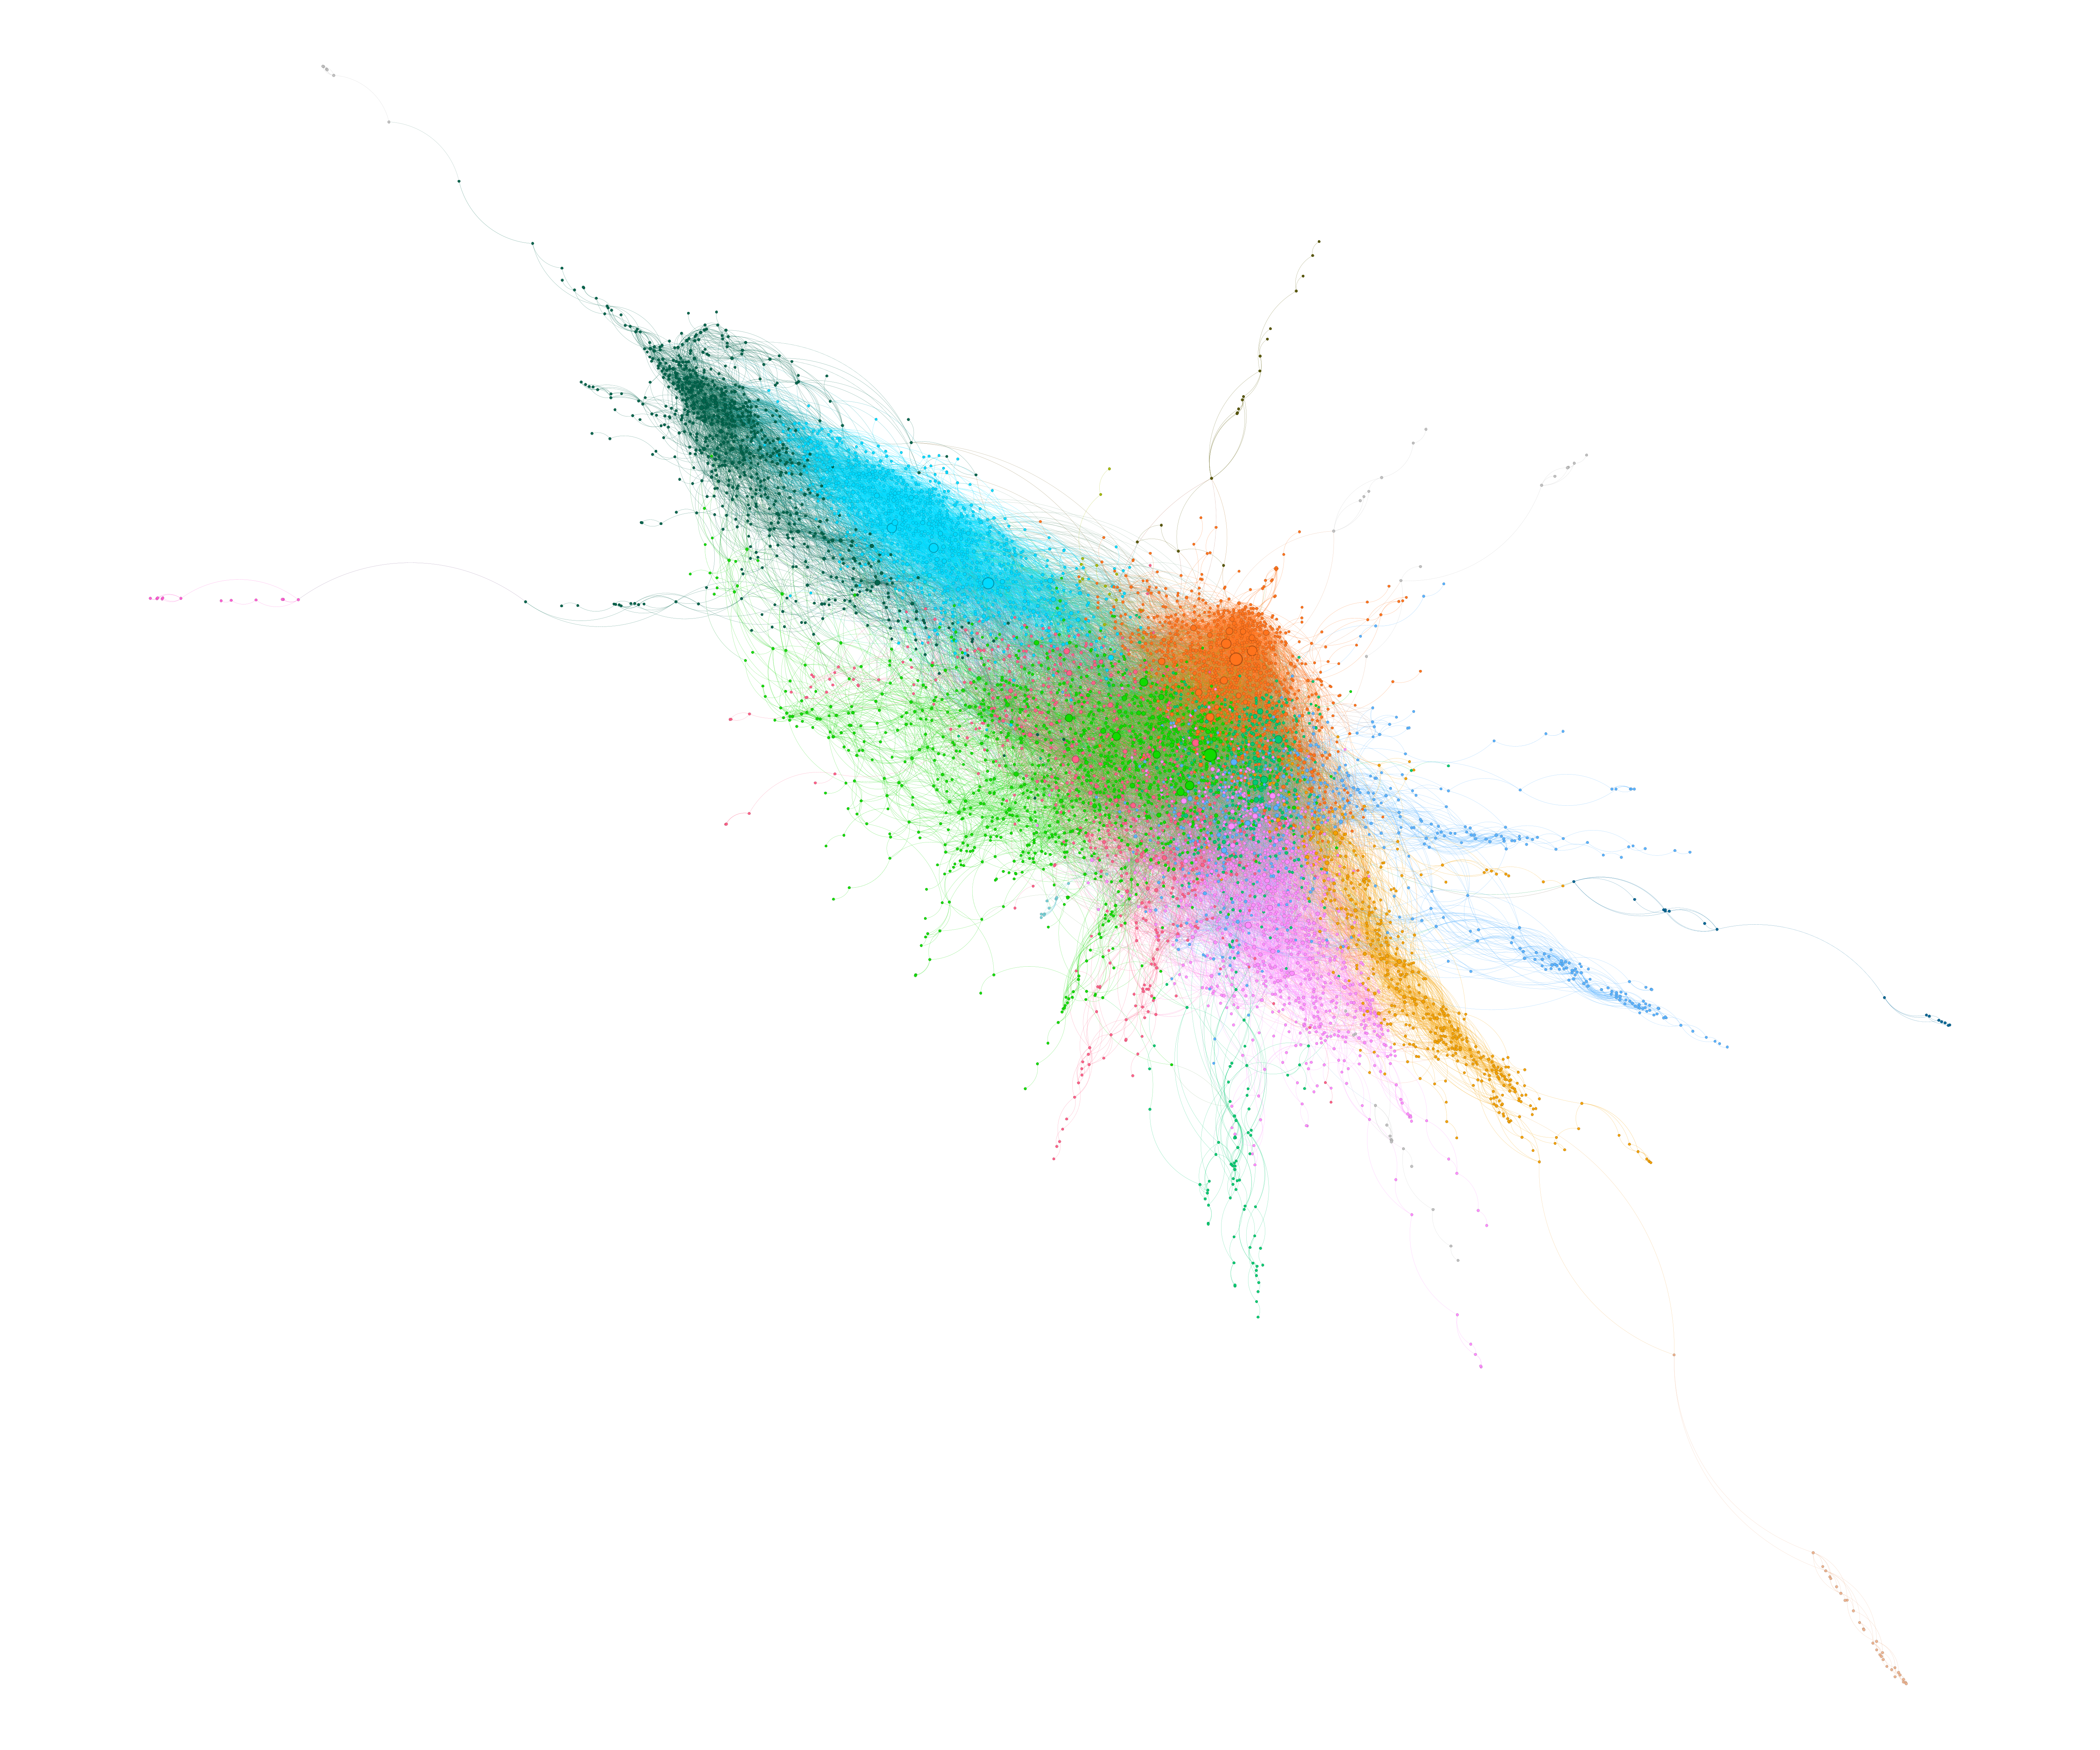
\includegraphics[width=\textwidth]{word2vec.png}
        \caption{Граф, полученный моделью Word2Vec}
        \label{fig:graph-word2vec}
    \end{subfigure}
    \begin{subfigure}[b]{0.4\textwidth}
        \centering
        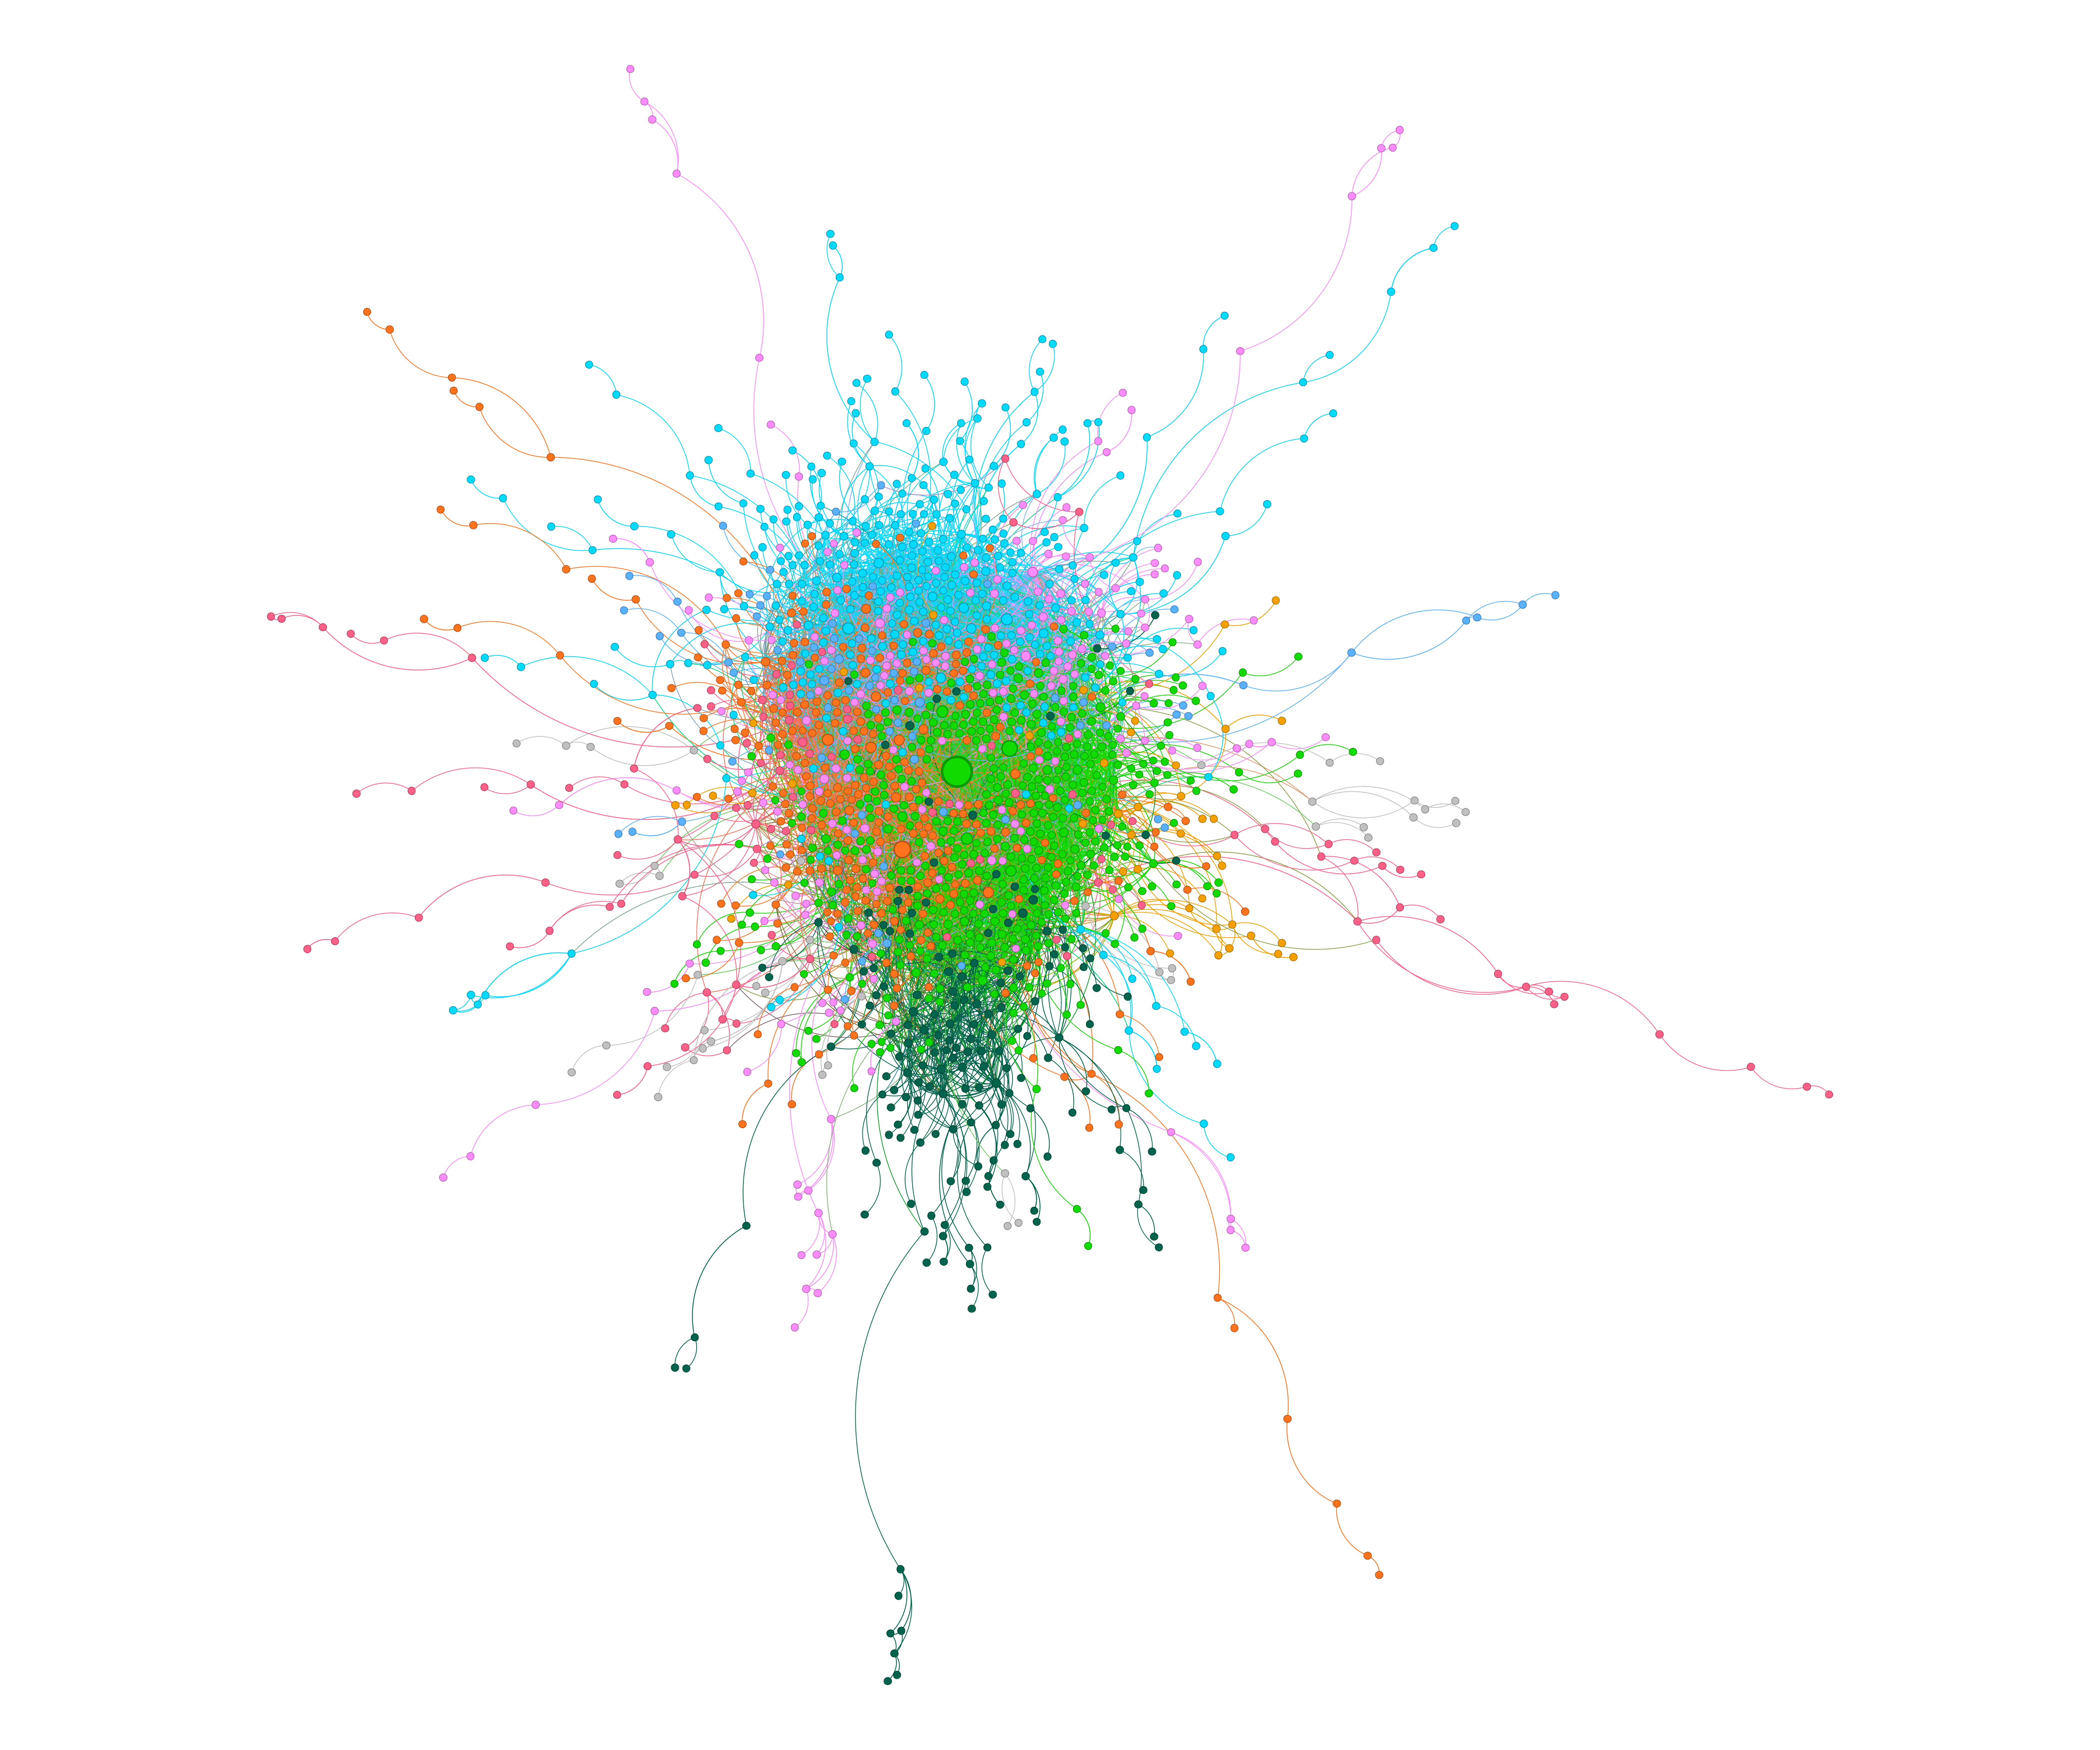
\includegraphics[width=\textwidth]{glove.png}
        \caption{Граф, полученный моделью GloVe}
        \label{fig:graph-glove}
    \end{subfigure}
    \caption{Графы, полученные моделями Word2Vec и GloVe}
\end{figure}

\subsection{Расширение моделей}
Ограниченный объём входных данных существенно сказывается на качестве получаемых векторных представлений. Модели, такие как Word2Vec или GloVe, эффективно обучаются только при наличии большого и разнообразного корпуса текстов, содержащего широкий спектр лексики и контекстов. В условиях малого корпуса наблюдаются следующие проблемы:
\begin{itemize}
    \item Слабое покрытие словаря: многие слова, особенно редкие или специфические для определённых тематик, могут вовсе не встретиться в обучающих данных. В результате модель не сможет построить для них эмбеддинги и они будут игнорироваться при дальнейшей обработке.

    \item Нестабильность эмбеддингов: даже для слов, входящих в корпус, контексты их употребления могут быть слишком ограниченными, чтобы обеспечить надёжную статистику. Это приводит к шумным или недостоверным векторным представлениям.

    \item Недостаточная семантическая выразительность: малая выборка не позволяет модели выявить устойчивые семантические закономерности между словами, что снижает эффективность таких задач, как кластеризация, классификация или семантический поиск.
\end{itemize}


Для решения данной проблемы возможно два подхода:
\begin{enumerate}
    \item Увеличение объёма обучающего корпуса, например, за счёт сбора дополнительных новостных текстов, включая архивные данные, региональные источники или тематические агрегаторы.
    
    \item Использование предварительно обученной модели (pretrained embeddings), полученной на большом и разнообразном корпусе (например, на Википедии, НКРЯ и т.д.), с последующим дообучением (fine-tuning) на новостных данных. Такой подход позволяет объединить общее языковое знание с контекстом конкретной предметной области.
\end{enumerate}
    
Возьмем модель\footnote{https://rusvectores.org/ru/models/} ruscorpora\_upos\_skipgram\_300\_5\_2018, которая была обучена на данных из НКРЯ, с объемом словаря равным $195 071$ слов. Эту модель будем сливать с моделью Word2Vec и отдельно с Glove, которые обучены на корпусе новостных документов.

Алгоритм получения эмбеддинга в модели, являющейся соединением модели ruscorpora\_upos\_skipgram\_300\_5\_2018 и модели Word2Vec или GloVe, следующий:
\begin{enumerate}
    \item Если эмбеддинг слова есть в обоих моделях, то используется среднее арифметическое векторов из обеих моделей.
    \item Если эмбеддинг слова есть только в одной из моделей, в итоговой модели используется вектор из той модели, в которой он имеется.
\end{enumerate}

С кодом, выполняющий выше описанный алгоритм, можно ознакомиться в приложении \ref{apx:thesaurus-expanding}:

\subsection{Получение эмбеддингов документов}
Для представления целого документа в векторном виде используется один из базовых и широко применяемых методов — усреднение эмбеддингов слов, входящих в данный документ. Суть подхода заключается в следующем: каждое слово в тексте заменяется своим вектором (эмбеддингом), после чего все эти векторы суммируются и результат делится на количество слов. Формально:
$$
    \bar{d} = \frac{1}{n} \sum_{i = 1}^n \bar{w}_i
$$
Полученные эмбеддинги документов сохраним в векторном индексе. С программным кодом можно ознакомиться в приложении \ref{apx:db}.

\subsection{Реализация алгоритма семантического поиска на основе корпуса новостей}

Перед началом поиска осуществляется загрузка векторных индексов, содержащих эмбеддинги документов, а также моделей эмбеддингов слов. Кроме того, загружается корпус новостных документов, создаётся отображение от идентификатора новости к её заголовку для последующего вывода результатов.

Алгоритм семантического поиска реализуется в несколько этапов:
\begin{enumerate}
    \item \textbf{Предварительная обработка пользовательского запроса.}
    Выполняется лемматизация и токенизация текста запроса:
    \begin{itemize}
        \item удаляются знаки препинания,
        \item производится приведение к нижнему регистру,
        \item слова приводятся к начальной форме с использованием \texttt{pymorphy3}.
    \end{itemize}

    \item \textbf{Получение эмбеддинга запроса.}
    Для каждого слова запроса, если оно содержится в выбранной модели, извлекается соответствующий эмбеддинг. Вектор запроса формируется как среднее арифметическое всех найденных векторов слов.

    \item \textbf{Поиск ближайших документов.}
    С помощью алгоритма ближайших соседей (k-NN), реализованного в \texttt{faiss}, осуществляется поиск наиболее релевантных документов на основе евклидовой метрики. По умолчанию возвращаются 5 наиболее близких документов.

    \item \textbf{Вывод результатов.}
    По найденным идентификаторам отображаются заголовки соответствующих новостей.
\end{enumerate}

С программным кодом, реализующим алгоритм семантического поиска можно ознакомиться в приложении \ref{apx:search}.

По данному алгоритму рассмотрим пример. В качестве запроса возьмём заголовок одной из новостей: \textit{<<В.В. Володин поздравил СГУ с праздником Победы>>}.

Результаты поэтапно:
\begin{enumerate}
    \item После предварительной обработки запроса получим список токенов:
    
    ['поздравить', 'сгу', 'праздник', 'победа']
    \item Преобразуем каждый токен в эмбеддинг через модель. Найдём среднее арифметические полученных эмбеддингов. В результате получим следующий эмбеддинг: 
    
    [[ 0.1731391   0.4556614   0.21552482  0.66046524, ...]]
    \item Найдём наиболее релевантные документы по полученному эмбеддингу. В результате получим идентификаторы новостей: 
    
    [22160, 2, 29536, 29551, 24466]
    \item Преобразуем идентификаторы новостей в их заголовки:
    \begin{itemize}
        \item В.В. Володин поздравил СГУ с праздником Победы, 
        \item СГУ приглашает саратовцев в парк Победы, 
        \item Н.В. Панков поздравляет коллектив СГУ с Новым годом,
        \item В.В. Володин поздравляет коллектив СГУ с днём Великой Победы,
        \item В СГУ пришли поздравления с майскими праздниками.
    \end{itemize}
\end{enumerate}

Далее идут примеры работы системы.

Пример 1:
\begin{minted}{text}
Запрос: май состояться общенародный акция бессмертный полк

First title should be: Студенты и сотрудники СГУ присоединились к шествию «Бессмертного полка»

Студенты и сотрудники СГУ присоединились к шествию «Бессмертного полка»
Балашовский институт принял участие в торжественных мероприятиях ко Дню Победы
Студенты СГУ приняли участие в акции, приуроченной ко Дню памяти и скорби
Делегация Саратовского университета прошла в строю «Бессмертного полка»
Студенты и сотрудники СГУ стали участниками мероприятий ко Дню Победы
\end{minted}

Видим, что самой близкой новостью является та, откуда был взять текст для запроса. Кромет того, заметим, что и другие новости довольно близки по значению к запросу.

Пример 2:
\begin{minted}{text}
Запрос: Вклад ученых

Ученые СГУ получили президентские гранты
В.С. Анищенко присвоено звание «Основатель научной школы»
Продолжается приём заявок на соискание премии Президента в области науки и инноваций
Учёный СГУ отмечен медалью ордена «За заслуги перед Отечеством» II степени
Фонд «БАЗИС» открыл приём заявок на конкурсы индивидуальных исследовательских грантов
\end{minted}

Пример 3:
\begin{minted}{text}
Запрос: Бессмертный полк

В СГУ открыт студенческий штаб акции «Бессмертный полк»
Сегодня в ИФиЖ состоится «Праздник белых журавлей»
Студенты и сотрудники СГУ стали участниками мероприятий ко Дню Победы
Сотрудники и студенты могут увековечить память защитников блокадного Ленинграда
Министерство молодёжной политики предлагает сделать 70 добрых дел
\end{minted}

Пример 4:
\begin{minted}{text}
Запрос: Чемпионат мира по программированию

СГУ участвует в проведении финала чемпионата ACM-ICPC 2013
Студент ИФКиС стал чемпионом России по кикбоксингу
Программисты СГУ отправились на финал Чемпионата мира
Профессор В.Н. Чинилов стал призёром Чемпионата России
В Саратове пройдёт Неделя информатики
\end{minted}

Можно заметить на последнем примере, что в ответе присутствуют новости, которые имеют опосредованное отношение к запросу (новость <<\textit{Студент ИФКиС стал чемпионом России по кикбоксингу}>> относится к запросу <<\textit{Чемпионат мира по программированию}>> лишь относительно слово \textit{чемпион}). Это может происходит из"=за трех причин:
\begin{enumerate}
    \item Простой способ получения эмбеддинга документа;
    \item Поиск $k$ ближайших документов алгоритмом осуществляется алгоритмом KNN (k-nearest neighbor);
    \item Эмбеддинги, получаемые из запроса, не учитывают контекст
\end{enumerate}

Однако, в среднем ответы на запрос действительно близки по смыслу к запросу, следовательно модель выдает релевантные документы. 

\section{Анализ работы семантического поиска на основе разных моделей}
Для качественного анализа была сгенерирована тестовая выборка, состоящая из пар: запрос и идентификатор новости. Считается, что модель справилась с задачей, если релевантная новость входит в первые $k$ результатов.

Запросы создавались с помощью модели \verb|microsoft/Phi-4-mini-instruct|, способной понимать русский язык. На вход ей подавался системный промпт и текст новости. Промпт ориентировал модель генерировать короткие, реалистичные и разнообразные запросы, имитируя поведение реальных пользователей. Промт имеет вид:
\begin{minted}{text}
Тебе дают текст новости. 
Сгенерируй 5 реалистичных поисковых запросов, которые могли бы ввести пользователи в поисковике, чтобы найти эту новость. 
Учитывай, что пользователи часто не знают точных формулировок, могут использовать ключевые слова, имена, места, приблизительные описания и синонимы. 
Запросы должны быть короткими (3-7 слов). Формулируй запросы разнообразно и естественно, как это делают реальные пользователи.
\end{minted}

Пример получаемого ответа:
\begin{minted}{text}
Саратовский конкурс «Сияние талантов» 2015, 
Юлиана Мелкумян, Саратовский университет, победитель вокала, Конкурс детского творчества в Саратове, Гран-при, 
Саратовский конкурс, вокалистка, поездка в Пекин, 
Конкурс «Сияние талантов», Саратов, награда в Пекине.
\end{minted}

С программным кодом можно ознакомиться в приложении \ref{apx:llm}.

Помимо запросов, сгенерированных с помощью LLM, были добавлены запросы, являющиеся заголовками новости.
Таким образом, сформировалась выборка из $3343$ запросов.

Результат работы семантического поиска на основе эмбеддингов моделей Word2Vec и Glove продемонстрированы на рис. \ref{fig:search-analyse}. Модель GloVe показывает более высокую точность: нужная новость оказывается на первом месте в $34\%$ запросов и входит в топ-5 в $38\%$ случаев. Для сравнения, модель Word2Vec выдаёт релевантную новость первой в $31\%$ запросов, а в топ-5 — в $35\%$.

Сравнение моделей Word2Vec и GloVe показало, что GloVe справляется лучше. Это объясняется тем, что GloVe обучается на глобальной статистике, что даёт ему преимущество в понимании семантики коротких запросов.

\begin{figure}[!ht]
    \centering
    \includegraphics[width=0.8\textwidth]{accuracy_by_model.png}
    \caption{Точность моделей Word2Vec и GloVe в задаче семантического поиска на основе корпуса новостей}
    \label{fig:search-analyse}
\end{figure}

\conclusion

В ходе выполнения курсовой работы была реализована система семантического поиска по корпусу новостных документов с использованием векторных представлений слов и текстов. Основной целью исследования являлось сопоставление качества поиска на основе двух популярных моделей эмбеддингов "--- Word2Vec и GloVe.

На первом этапе была проведена теоретическая проработка алгоритмов построения эмбеддингов, а также изучено понятие <<информационно"=поискового тезауруса>>. Далее были построены модели Word2Vec и GloVe на специально собранном корпусе новостных текстов. Затем реализован алгоритм семантического поиска, использующий векторные представления как для пользовательских запросов, так и для документов.

Особое внимание было уделено созданию тестовой выборки, включающей как реальные заголовки новостей, так и запросы, сгенерированные с помощью крупной языковой модели (LLM). Это позволило сформировать разнообразную и реалистичную среду для оценки эффективности семантического поиска.

Анализ результатов показал, что модель GloVe превосходит Word2Vec по точности выдачи релевантных результатов. В частности, GloVe возвращает нужную новость на первом месте в $34\%$ случаев, а в топ-5 — в $38\%$, тогда как Word2Vec — соответственно в $31\%$ и $35\%$. Кроме того, модель Word2Vec склонна выдавать больше нерелевантных и <<шумных>>  ближайших соседей, особенно при работе с абстрактными понятиями.

Таким образом, можно сделать вывод, что использование эмбеддингов, основанных на глобальной статистике, таких как GloVe, более предпочтительно для задач семантического поиска по новостным документам. Такая модель лучше улавливает смысловые связи между короткими пользовательскими запросами и содержанием новостей, что особенно важно в условиях информационного шума и вариативности формулировок.

% Отобразить все источники. Даже те, на которые нет ссылок.
% \nocite{*}
\inputencoding{cp1251}
\bibliographystyle{gost780uv}
\bibliography{thesis}
\inputencoding{utf8}

% Окончание основного документа и начало приложений Каждая последующая секция
% документа будет являться приложением
\setminted[python3]{fontsize=\footnotesize, breaklines=true, style=bw, linenos}
\appendix
\section{Программный код, выполняющий обработку текста}
\label{apx:tokenization}
\begin{minted}{python3}
import pandas as pd
import pymorphy3
import re
import dask.dataframe as dd
def string_dev(a_in):
    x_in = re.sub(r'\n', ' ', a_in)
    y_in = x_in.lower()
    b_in = re.sub(r'&\w+;', ' ', y_in)
    d_in = re.sub(r'<[^>]*>', ' ', b_in)
    f_in = re.sub(r'www\.\w+\.\w{2,3}?', ' ', d_in)
    a_in = re.sub(r'\xad', '', f_in)
    c_in = re.sub(r'\\xa0-', '', a_in)
    u_in = re.sub(r'\\u200e', '', c_in)
    w_in = re.sub(r'\d+', '', u_in)
    y_in = re.sub(r'\-', ' ', w_in)
    yy_in = re.sub(r'_+', ' ', y_in)
    yyy_in = re.sub(r'[…"---–/()"\[\]\\\\,\-:;<>©@№#%\'\+\*“”&~\$\^«»_і‑]+', '', yy_in)
    q_in = re.sub(r'[a-z]*', '', yyy_in)
    sss_in = re.sub(r'\b\w{,2}\b', '', q_in)
    qms_in = re.sub(r'\s{2,}', ' ', sss_in)
    nms_in = qms_in.strip()
    return nms_in
def lematization(f_input_list):
    morph = pymorphy3.MorphAnalyzer()
    lnorm = []
    for word in f_input_list:
        p = morph.parse(word)[0]
        lnorm.append(p.normal_form)
    return lnorm
def del_my_stop_words(word_tokens):
    stop_words = {
        'который', 'кому', 'имя', 'сегодня', 'вчера', 'завтра', 'также', 'в', 'во', 
        'свой', 'это', 'часто','зачастую', 'мочь', 'смочь', 'а', 'без', 'более', 
        'больше', 'будет', 'ведь', 'вот', 'впрочем', 'все','всегда', 'всего', 
        'всех', 'всю', 'вы', 'где', 'с', 'со', 'сам', 'свою', 'себе', 'себя', 
        'сейчас', 'c','совсем', 'так', 'такой', 'там', 'тебя', 'тем', 'теперь', 
        'то', 'тогда', 'того', 'тоже', 'только','том', 'тот', 'три', 'тут', 'ты', 
        'у', 'уж', 'уже', 'хорошо', 'хоть', 'что', 'чего', 'чем', 'через','чтоб', 
        'чтобы', 'чуть', 'эти', 'этого', 'этой', 'этом', 'этот', 'эту', 'я','сгт', 
        'стать', 'кроме', 'разный', 'около', 'затем', 'помимо', 'ваш', 'вам', 
        'некоторый', 'лишь','каждый', 'самый', 'неоднократно', 'ещё', 'сразу', 
        'среди', 'однако', 'вновь', 'иной', 'ныне', 'пока','хотя', 'либо', 
        'немного', 'гораздо', 'ничто', 'нередко', 'наоборот', 'впереди', 'таковой', 
        'мимо','тесно', 'вряд', 'нечто', 'почём', 'почему', 'любой', 'обратно', 
        'оттуда', 'очень', 'понапрасну','поскольку', 'поэтому', 'прежде', 'причём', 
        'прочий', 'пусть', 'наш', 'несколько', 'никак', 'твой','подробный', 
        'информация'
    }
    return [w for w in word_tokens if w not in stop_words]
from natasha import Segmenter, MorphVocab, NewsEmbedding, NewsMorphTagger, NewsNERTagger, Doc
segmenter = Segmenter()
morph_vocab = MorphVocab()
emb = NewsEmbedding()
morph_tagger = NewsMorphTagger(emb)
ner_tagger = NewsNERTagger(emb)
def remove_proper_nouns(text):
    if not isinstance(text, str) or not text.strip():
        print("text имеет неожидаемый тип")
        return "error type"
    try:
        doc = Doc(text)
        doc.segment(segmenter)
        doc.tag_morph(morph_tagger)
        doc.tag_ner(ner_tagger)
        if not doc.spans:
            return text
        spans_to_remove = [span for span in doc.spans if span.type in ['PER', 'LOC', 'ORG']]
        text_cleaned = text
        for span in sorted(spans_to_remove, key=lambda x: x.start, reverse=True):
            text_cleaned = text_cleaned[:span.start] + text_cleaned[span.stop:]
        print(text_cleaned)
        return text_cleaned.strip()
    except Exception as e:
        print(f"Ошибка при обработке текста: {text[:50]}... Ошибка: {str(e)}")
        return "error"
def process_str_of_the_news(string):
    string_2 = string_dev(string)
    if len(string_2) != 0:
        list_of_sentences = re.split(r'[.!?]', string_2)
        list_of_sentences = [x.split(' ') for x in list_of_sentences if x]
        filtered_sentences = []
        for sentence in list_of_sentences:
            no_stopwords_1 = del_my_stop_words(sentence)
            lemmatized = lematization(no_stopwords_1)
            text = ' '.join(lemmatized)
            text = re.sub(r'\b\w{1,2}\b', '', text)
            text = re.sub(r'\s{2,}', ' ', text)
            text = text.strip()
            if text:
                filtered_sentences.append(text)
    return filtered_sentences
import pyarrow as pa
def apply_tokenization():
    docs = dd.read_parquet("raw-data.pq").repartition(npartitions=8).loc[:1]
    print("Read finished")
    docs['News_Tokens'] = docs['News_Text'].map_partitions(
        lambda s: s.apply(remove_proper_nouns),
        meta=("News_Tokens", object)
    )
    docs['News_Tokens'] = docs["News_Tokens"].map_partitions(
        lambda s: s.apply(process_str_of_the_news),
        meta=("News_Tokens", object)
    )
    print("Returning")
    schema = {
        "News_Text": pa.string(),
        "News_Tokens": pa.list_(pa.string()),
        "News_Title": pa.string()
    }
    return docs.to_parquet("output.pq", schema=schema, write_metadata_file=True)
apply_tokenization()
\end{minted}
\section{Построение тезауруса по модели эмбеддинга}
\label{apx:thesaurus}
\begin{minted}{python3}
import pandas as pd
import dask.dataframe as dd
import dask.bag as db
from gensim.models import Word2Vec
docs = dd.read_parquet("../output.pq/")
model = Word2Vec.load("word2vec_sent_5_sgu.model")
texts = docs['News_Tokens'].compute()
bag = db.from_sequence(texts)
sentences = bag.flatten()
words = sentences.map(lambda x: x.split()).flatten().distinct()compute()
results = []
threshold = 0.8
for word in words:
    try:
        # Получаем 10 ближайших слов
        similar_words = model.wv.most_similar(word, topn=10)
        filtered_words = [(w, sim) for w, sim in similar_words if sim >= threshold]
        results.append([word, filtered_words])
    except KeyError:
        # Если слово не в модели, пропускаем его
        print(f"Слово '{word}' не найдено в модели.")

df_results = pd.DataFrame(results, columns=["Word","Most_Similar_Word"])
df_results.to_csv("similar_words_sent_5.csv", index=False)
\end{minted}
\section{Получение случайных 20 слов}
\label{apx:cherrypick}
\begin{minted}{python3}
import pandas as pd
import os
file_paths = {
    'glove': '/glove_python/sim-words_sent_5_glove.csv',
    'word2vec': '/word2vec/similar_words_sent_5.csv'
}
data = pd.DataFrame(columns=['word'])
for model_name, path in file_paths.items():
    full_path = ".." + path
    df = pd.read_csv(full_path)
    df = df.rename(columns={'Most_Similar_Word': model_name})
    if data.empty:
        data['word'] = df['Word']
    data[model_name] = df[model_name]
import ast
def is_valid_similar_words(value):
    if pd.isna(value):
        return False
    if isinstance(value, str):
        try:
            lst = ast.literal_eval(value)
            return len(lst) > 0
        except (ValueError, SyntaxError):
            return False
    elif isinstance(value, list):
        return len(value) > 0
    else:
        return False
filtered_data = data[
    data['glove'].apply(is_valid_similar_words) &
    data['word2vec'].apply(is_valid_similar_words)
]
n = 25  # кол-во случайных строк
random_sample = filtered_data.sample(n=n, random_state=42)
output_file = 'random_sample_similar_words.csv'
random_sample.to_csv(output_file, index=False, encoding='utf-8')
\end{minted}

\section{Построение графа}
\label{apx:graph}
\begin{minted}{python3}
import pandas as pd
import networkx as nx
from ast import literal_eval
file_paths = {
    'glove': '/glove_python/sim-words_sent_5_glove.csv',
    'word2vec': '/word2vec/similar_words_sent_5.csv'
}
data = {}
for model_name, path in file_paths.items():
  df = pd.read_csv(".." + path)
  data[model_name] = df
graphs = {}
for model_name, df in data.items():
    G = nx.Graph()
    for _, row in df.iterrows():
        word = row['Word']
        similar_words = row['Most_Similar_Word']
        if not similar_words or pd.isna(similar_words):
            continue
        try:
            similar_words = literal_eval(similar_words)
        except (ValueError, SyntaxError):
            continue
        for similar_word, weight in similar_words:
            G.add_edge(word, similar_word, weight=weight)
    graphs[model_name] = G    
    nx.write_gexf(G, f"{model_name}_graph.gexf")
    print(f"Граф '{model_name}' {len(G.nodes)} {len(G.edges)}")
from community import community_louvain
for model_name, G in graphs.items():
  print(f"model name: {model_name}")
  partition = community_louvain.best_partition(G, weight='weight')
  num_clusters = max(partition.values()) + 1
  print(f"Число кластеров (Louvain): {num_clusters}")
  from collections import Counter
  cluster_sizes = Counter(partition.values())
  print(f"Размеры кластеров: {cluster_sizes.most_common(5)}")
  modularity = community_louvain.modularity(partition, G, weight='weight')
  print(f"Модулярность: {modularity:.3f}")
\end{minted}
\section{Расширение модели, построенной на корпусе новостных документов}
\label{apx:thesaurus-expanding}
\begin{minted}{python3}
from gensim.models import KeyedVectors
big = KeyedVectors.load_word2vec_format("ruscorpora_upos_skipgram_300_5_2018/model.vec", binary=False)
small = KeyedVectors.load("word2vec_sent_5_sgu.vec") // and glove_sent_5_sgu.model
small_words = set(small.wv.key_to_index.keys())
big_words = set(big.key_to_index.keys())
all_words = small_words.union(big_words)
new_vocab = {}
new_vectors = []
for word in all_words:
    if word in small_words and word in big_words:
        vec = (small.wv[word] + big.get_vector(word)) / 2
    elif word in small_words:
        vec = small.wv[word]
    else:
        vec = big.get_vector(word)
    new_vocab[word] = len(new_vectors)
    new_vectors.append(vec)
new_kv = KeyedVectors(vector_size=big.vector_size)
new_kv.add_vectors(list(new_vocab.keys()), new_vectors)
new_kv.save("word2vec.kv")
\end{minted}
\section{Получение и сохранение эмбеддингов документов}
\label{apx:db}
\begin{minted}{python3}
import pandas as pd
from gensim.models import KeyedVectors
import dask.dataframe as dd
import dask.bag as db
import numpy as np
import json
import faiss
# Пути к файлам
file_paths = {
    'glove': '../glove_python/glove.kv', 
    'word2vec': '../word2vec/word2vec.kv'
}
word2vec = KeyedVectors.load(file_paths['word2vec'], mmap='r')
glove = KeyedVectors.load(file_paths['glove'],  mmap='r')
docs = dd.read_parquet("../output.pq/")
texts = docs['News_Tokens'].compute()
bag = db.from_sequence(texts)
list_news = bag.map(lambda sent: ' '.join(sent)).map(lambda news: news.split()).compute()
ids = docs['News_Id'].compute()
def get_doc_embedding(tokens, model):
    vectors = [model[word] for word in tokens if word in model]
    if vectors:
        return np.mean(vectors, axis=0)
    else:
        return np.zeros(model.vector_size)
glove_embeddings = {}
word2vec_embeddings = {}
for (news, id) in zip(list_news, ids):
  word2vec_embeddings[id] = get_doc_embedding(news, word2vec)
  glove_embeddings[id] = get_doc_embedding(news, glove)
folder = 'news-embeddings'
def save_embeddings_dict(emb_dict, prefix):
    ids = list(emb_dict.keys())
    vectors = np.array([emb_dict[i] for i in ids], dtype='float32')
    index = faiss.IndexFlatL2(vectors.shape[1])
    index.add(vectors)
    np.save(f"{folder}/{prefix}_vectors.npy", vectors)
    faiss.write_index(index, f"{folder}/{prefix}.index")
    with open(f"{folder}/{prefix}_ids.json", "w", encoding="utf-8") as f:
        json.dump(ids, f)
save_embeddings_dict(glove_embeddings, "glove")
save_embeddings_dict(word2vec_embeddings, "word2vec")
\end{minted}
\section{Реализация алгоритма семантического поиска}
\label{apx:search}
\begin{minted}{python3}
import numpy as np
import json
import faiss

def load_index_and_ids(prefix: str, folder: str = "news-embeddings"):
    # Загрузка FAISS индекса
    index = faiss.read_index(f"{folder}/{prefix}.index")
    
    # Загрузка соответствующих ID
    with open(f"{folder}/{prefix}_ids.json", "r", encoding="utf-8") as f:
        ids = json.load(f)
    
    return index, ids
db = {
  "glove": load_index_and_ids("glove"),
  "word2vec": load_index_and_ids("word2vec")
}
from gensim.models import KeyedVectors
models = {
  "glove": KeyedVectors.load("../glove_python/glove.kv"),
  "word2vec": KeyedVectors.load("../word2vec/word2vec.kv")
}
# Считывание новостей
import dask.dataframe as dd
docs = dd.read_parquet("../output.pq/", columns=['News_Id', 'News_Title', 'News_Tokens'])
df = docs.compute()
id_to_title = dict(zip(df['News_Id'], df['News_Title']))
import pymorphy3
import re
def lematization(f_input_list):          # Лематизация слов в списке
    morph = pymorphy3.MorphAnalyzer()
    lnorm = list()
    for word in f_input_list:
        p = morph.parse(word)[0]
        lnorm.append(p.normal_form)
    return (lnorm)
def preprocess_query(query):
    query = query.lower()
    query = re.sub(r"[^\w\s]", " ", query)
    query = re.sub(r'\b\w{,2}\b','', query)
    query = re.sub(r'\s{2,}', ' ', query)
    tokens = query.split()
    return lematization(tokens)
def get_query_embedding(query: str, model_name: str):
    model: KeyedVectors = models[model_name]
    tokens = preprocess_query(query=query)
    # print(f"tokens = {tokens}")
    vectors = [model[word] for word in tokens if word in model]
    if not vectors:
        print(f"Query vector {query} is empty")
        return np.zeros((1, model.vector_size), dtype='float32')
    return np.mean(vectors, axis=0).astype('float32').reshape(1, -1)
def semantic_search(query: str, model_name: str, k = 5):
    query_vec = get_query_embedding(query, model_name)
    # print(f"query_vec = {query_vec}")
    if np.linalg.norm(query_vec) == 0:
        return []
    index, ids = db[model_name]
    D, I = index.search(query_vec, k)
    news_ids = [ids[i] for i in I[0]]
    # print(f"Result_index = {news_ids}")
    return news_ids
text = "..." # input there
answers = semantic_search(query=text, model_name="word2vec")
answers = [id_to_title[i] for i in answers]
for answer in answers:
  print(answer)
\end{minted}
\section{Генерация запросов LLM}
\label{apx:llm}
\begin{minted}{python3}
from transformers import pipeline
import re
chatbot = pipeline("text-generation", model="microsoft/Phi-4-mini-instruct", max_new_tokens=256)
def parse_queries(llm_q: str) -> list[str]:
    # Разбиваем по строкам
    lines = llm_q.strip().split('\n')
    queries = []
    for line in lines:
        # Убираем номер и точку в начале строки, например "1. "
        query = re.sub(r'^\s*\d+\.\s*', '', line)
        queries.append(query.strip())
    return queries
promt_template = lambda news: f"""Вот текст новости:\n{news}"""
def generate_query(text: str) -> list[str]:
    messages = [
        {"role": "system", "content": """Тебе дают текст новости. 
         Сгенерируй 5 реалистичных поисковых запросов, которые могли бы ввести пользователи в поисковике, чтобы найти эту новость. 
         Учитывай, что пользователи часто не знают точных формулировок, могут использовать ключевые слова, имена, места, приблизительные описания и синонимы. 
         Запросы должны быть короткими (3-7 слов). Формулируй запросы разнообразно и естественно, как это делают реальные пользователи."""},
        {"role": "user", "content": promt_template(text)}
    ]
    llm_q = chatbot(messages)[0]['generated_text'][2]['content']
    return parse_queries(llm_q)
sample_df = docs.sample(frac=0.0001, random_state=42)
sample_df['News_Query'] = sample_df['News_Text'].map(generate_query,  meta=("News_Tokens", object)).compute()
import pyarrow as pa
schema = {
        "News_Id": pa.int64(),
        "News_Text": pa.string(),
        "News_Title": pa.string(),
        "News_Query": pa.string()
    }
sample_df.to_csv('llm-query.pq')
\end{minted}
\end{document}
  